\documentclass[tikz,border=5pt]{standalone}
\usepackage{amsmath}
\usetikzlibrary{calc}
\begin{document}
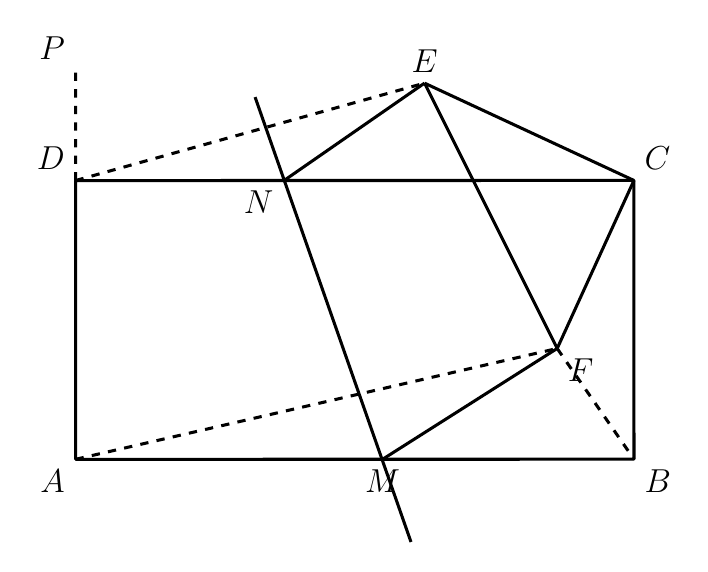
\begin{tikzpicture}[line width=1.1pt, line join=round,
  lbl/.style={font=\fontsize{11.5}{13.8}\selectfont}]
  % Named coordinates (pixel -> units, y flipped, scale 1/100)
  \coordinate (A) at (0.00048153937484940457,0.00012725477801023288);
  \coordinate (B) at (7.091927141940605,0.0013353788423469126);
  \coordinate (C) at (7.091324025170966,3.541509678938571);
  \coordinate (D) at (-0.00012157739479023988,3.5403015548742345);
  \coordinate (E) at (4.431777666534905,4.777436234815082);
  \coordinate (N) at (2.648222641998573,3.5407527362780566);
  \coordinate (M) at (3.899999865141729,0.0007915906825224361);
  \coordinate (F) at (6.116748732256346,1.4077456321280535);
  \coordinate (P) at (-0.0003600350231836025,4.939999938663123);
  % Fold line endpoints
  \coordinate (FoldTop) at (2.28,4.6);
  \coordinate (FoldBot) at (4.26,-1.05);

  % Rectangle ABCD
  \draw (A) -- (B) -- (C) -- (D) -- cycle;

  % Fold line through N and M
  \draw (FoldTop) -- (FoldBot);

  % Solid segments
  \draw (E) -- (N);
  \draw (E) -- (C);
  \draw (E) -- (F);
  \draw (F) -- (C);
  \draw (F) -- (M);

  % Dashed segments
  \draw[dashed] (D) -- (E);
  \draw[dashed] (A) -- (F);
  \draw[dashed] (F) -- (B);
  \draw[dashed] (D) -- (P);

  % Labels
  \node[lbl, below left] at (A) {$A$};
  \node[lbl, below right] at (B) {$B$};
  \node[lbl, above right] at (C) {$C$};
  \node[lbl, above left] at (D) {$D$};
  \node[lbl, above] at (E) {$E$};
  \node[lbl, below left] at (N) {$N$};
  \node[lbl, below] at (M) {$M$};
  \node[lbl, below right] at (F) {$F$};
  \node[lbl, above left] at (P) {$P$};
\end{tikzpicture}
\end{document}